\subsection{Parallelisierung}
Zur Parallelisierung des Merge-Sort Algorithmus wird aufgrund beschränkter Zeit ein vereinfachter Algorithmus verwendet.\\
Die zu sortierenden Daten werden auf der Master Node in gleich große Vektoren gespaltet, welche erneut in einem Vektor verwaltet werden. Die Anzahl der Vektoren entspricht der Anzahl der verfügbaren Nodes und der Datensatz wird unsortiert möglichst gleich auf die Vektoren verteilt. Eine Konvertierung von einem Vektor von Strings in ein großes Char-Array mit Trennzeichen ermöglicht die Übertragung des Datensatzes, welcher für den jeweiligen Worker bestimmt ist, in einer einzigen Nachricht. 
\\
Auf den Workern werden die Char-Arrays wieder in Vektoren von Strings umgewandelt, was die Verwendung der bestehenden Implementierung des Merge-Sort Algorithmus ermöglicht. Der sortierte Vektor, welcher das Ergebnis des Merge-Sorts ist, wird erneut über Umwandlung in ein Char-Array zurück zur Master Node geschickt. Auf der Master Node wird nach Erhalt der Ergebnisse aller Worker diese zusammengeführt und als Ergebnis Vektor ausgegeben. Zur Zusammenführung der Daten werden jeweils die ersten beiden Vektoren aus dem Vektor entfernt und mit der bestehenden Merge Funktion zusammengeführt. Daraus wird erneut ein Vektor gebildet, welcher an das Ende des Ergebnisvektors angehängt wird. Dieser Algorithmus wird ausgeführt bis die Elemente des Ergebnisvektors auf Eins reduziert wurden. Das Element des Ergebnisvektors wird nun als Endergebnis ausgegeben und enthält die sortierten Daten. 
\\
\begin{figure}[!t]
	\centering
	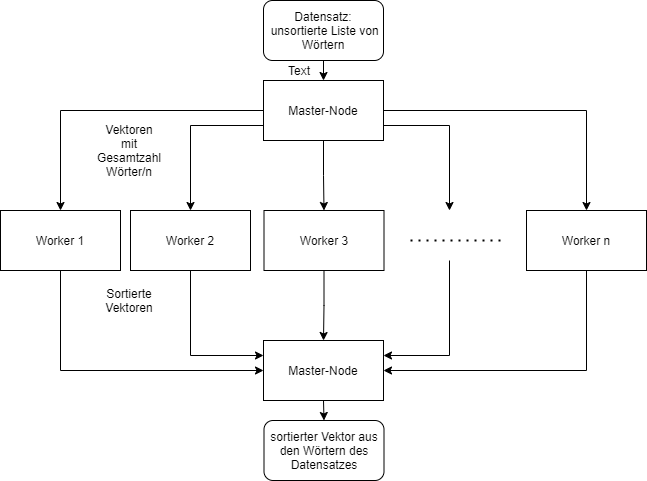
\includegraphics[width=3.5in]{Parallelisierungs_Algorithmus.png}
	\caption{Datenfluss des implementierten Algorithmus}
	\label{para_algo1}
\end{figure}
Basierend auf der Aufteilung kann eine undefinierte Anzahl von Nodes verwendet werden. Die Sortierung der Teil Vektoren wird hierbei immer von allen Nodes einschließlich dem Master übernommen.
\\

